\chapter{Hybrid FGTN-Mamba: phương pháp đề xuất}
\label{ch:method}

Chương này mô tả khối Hybrid FGTN-Mamba và pipeline phát hiện hoàn chỉnh. Mọi mô tả bám theo cài đặt trong thư mục \path{projects/fgtn_ava} của kho mã; các siêu tham số nêu dưới đây là giá trị thực tế trong cấu hình huấn luyện.

\section{Tổng quan kiến trúc}
\label{sec:overview}

Pipeline đề xuất (\cref{fig:pipeline}) gồm năm bước:
\begin{enumerate}
  \item Backbone Video Swin-Tiny \cite{liu2022videoswin}, tiền huấn luyện trên Kinetics-400, trích đồng thời bản đồ đặc trưng của tầng 3 và tầng 4.
  \item Mỗi tầng đi qua một Hybrid FGTN-Mamba riêng, với tham số phù hợp độ phân giải và mức ngữ nghĩa của tầng đó, để đặc trưng được làm giàu theo thời gian trước khi cắt theo person proposal.
  \item 3D RoIAlign lấy đặc trưng của từng person proposal ở cả hai tỉ lệ rồi nối theo kênh (multi-scale RoI): tầng 3 giữ chi tiết như điện thoại, bàn tay, bàn chân; tầng 4 giữ ngữ nghĩa toàn thân.
  \item ACRN học quan hệ giữa từng actor với bàn, ghế, thiết bị và cảnh xung quanh.
  \item Head sigmoid dự đoán xác suất độc lập cho từng nhãn, huấn luyện bằng focal loss kết hợp trọng số lớp; khi suy luận, ngưỡng theo lớp và logic theo track giảm cảnh báo chớp tắt.
\end{enumerate}

Thành phần mới trung tâm là Hybrid FGTN-Mamba (bước 2); đặc trưng đa tỉ lệ, ACRN và hàm mất mát hai cấp là các thành phần có tiền lệ, được tích hợp để xử lý các hạn chế còn lại (\cref{sec:multiscale,sec:acrn,sec:loss}). Các tầng của Video Swin-T được đánh số từ 1 đến 4 như \cref{fig:architecture}; tầng 3 và tầng 4 tương ứng \code{out\_indices} 2 và 3 trong mã nguồn (``stage 2'' và ``stage 3'' khi đánh số từ 0). Với đoạn video $V \in \R^{3 \times 32 \times 256 \times 256}$ và $N$ hộp người, chuỗi biến đổi của pipeline đầy đủ là
\begin{equation}
\begin{aligned}
V &\xrightarrow{\text{Swin-T}} \big(F^{(3)}, F^{(4)}\big)
  \xrightarrow{\text{HFM}_3,\ \text{HFM}_4} \big(\tilde{F}^{(3)}, \tilde{F}^{(4)}\big)\\
  &\xrightarrow{\text{RoIAlign}} r_k
  \xrightarrow{\text{ACRN}} c_k
  \xrightarrow{\text{head}} \mat{p}_k \in [0,1]^{K},
\end{aligned}
\label{eq:flow}
\end{equation}
trong đó $F^{(3)} \in \R^{384 \times 16 \times 16 \times 16}$, $F^{(4)} \in \R^{768 \times 16 \times 8 \times 8}$, $\text{HFM}_s$ là ngăn xếp hai khối Hybrid FGTN-Mamba của tầng $s$, $r_k \in \R^{1152 \times 1 \times 8 \times 8}$ là đặc trưng RoI đa tỉ lệ và $c_k$ là đầu ra của ACRN. Biến thể một tỉ lệ (cấu hình A6 trong \cref{tab:ablation}) bỏ tầng 3 và ACRN: $V \rightarrow F^{(4)} \rightarrow \tilde{F}^{(4)} \rightarrow r_k \in \R^{768 \times 1 \times 8 \times 8} \rightarrow \mat{p}_k$.

\begin{figure}[H]
\centering
\resizebox{\textwidth}{!}{%
\begin{tikzpicture}[font=\footnotesize, >={Stealth[length=2mm]},
  blk/.style={draw, rounded corners=2pt, align=center, inner sep=3pt,
              minimum height=10mm, line width=0.6pt},
  arr/.style={->, line width=0.7pt}]
  \node[blk, fill=blue!7, minimum width=17mm, minimum height=32mm] (swin)
    {Video\\Swin-T\\[3pt]{\scriptsize tiền huấn}\\{\scriptsize luyện K400}};
  \node[blk, fill=orange!14, minimum width=29mm, anchor=west] (h3)
    at ($(swin.east)+(21mm,9mm)$) {Hybrid FGTN-Mamba\\{\scriptsize tham số riêng tầng 3}};
  \node[blk, fill=orange!14, minimum width=29mm, anchor=west] (h4)
    at ($(swin.east)+(21mm,-9mm)$) {Hybrid FGTN-Mamba\\{\scriptsize tham số riêng tầng 4}};
  \draw[arr] ($(swin.east)+(0,9mm)$) --
    node[above, font=\scriptsize] {tầng 3}
    node[below, font=\scriptsize] {$C{=}384$, $\tfrac{1}{16}$} (h3.west);
  \draw[arr] ($(swin.east)+(0,-9mm)$) --
    node[above, font=\scriptsize] {tầng 4}
    node[below, font=\scriptsize] {$C{=}768$, $\tfrac{1}{32}$} (h4.west);
  \coordinate (mid) at ($(h3.east)!0.5!(h4.east)$);
  \node[blk, fill=green!10, minimum width=22mm, anchor=west] (roi) at ($(mid)+(10mm,0)$)
    {RoIAlign 3D\\đa tỉ lệ\\{\scriptsize nối kênh $384{+}768$}};
  \draw[arr] (h3.east) -- ++(5mm,0) |- ($(roi.west)+(0,2.5mm)$);
  \draw[arr] (h4.east) -- ++(5mm,0) |- ($(roi.west)+(0,-2.5mm)$);
  \node[blk, fill=gray!8, above=6mm of roi] (prop) {Person proposal};
  \draw[arr] (prop) -- (roi);
  \node[blk, fill=green!10, right=6mm of roi] (acrn) {ACRN\\{\scriptsize actor--cảnh}};
  \node[blk, fill=magenta!8, right=6mm of acrn] (head) {Head\\sigmoid\\{\scriptsize đa nhãn}};
  \node[blk, fill=gray!8, right=6mm of head] (alert) {Ngưỡng theo lớp\\+ logic theo track\\$\Rightarrow$ cảnh báo};
  \draw[arr] (roi) -- (acrn);
  \draw[arr] (acrn) -- (head);
  \draw[arr] (head) -- (alert);
\end{tikzpicture}}
\caption[Pipeline phát hiện đầy đủ]{Pipeline phát hiện đầy đủ: Video Swin-T trích đặc trưng tầng 3 (384 kênh, bước 16) và tầng 4 (768 kênh, bước 32); mỗi tầng qua một Hybrid FGTN-Mamba với tham số riêng; RoIAlign 3D lấy đặc trưng của từng person proposal ở hai tỉ lệ và nối theo kênh; ACRN bổ sung quan hệ actor--cảnh; head sigmoid cho điểm từng hành vi; ngưỡng theo lớp và logic theo track quyết định việc phát cảnh báo.}
\label{fig:pipeline}
\end{figure}

\begin{figure}[htbp]
\centering
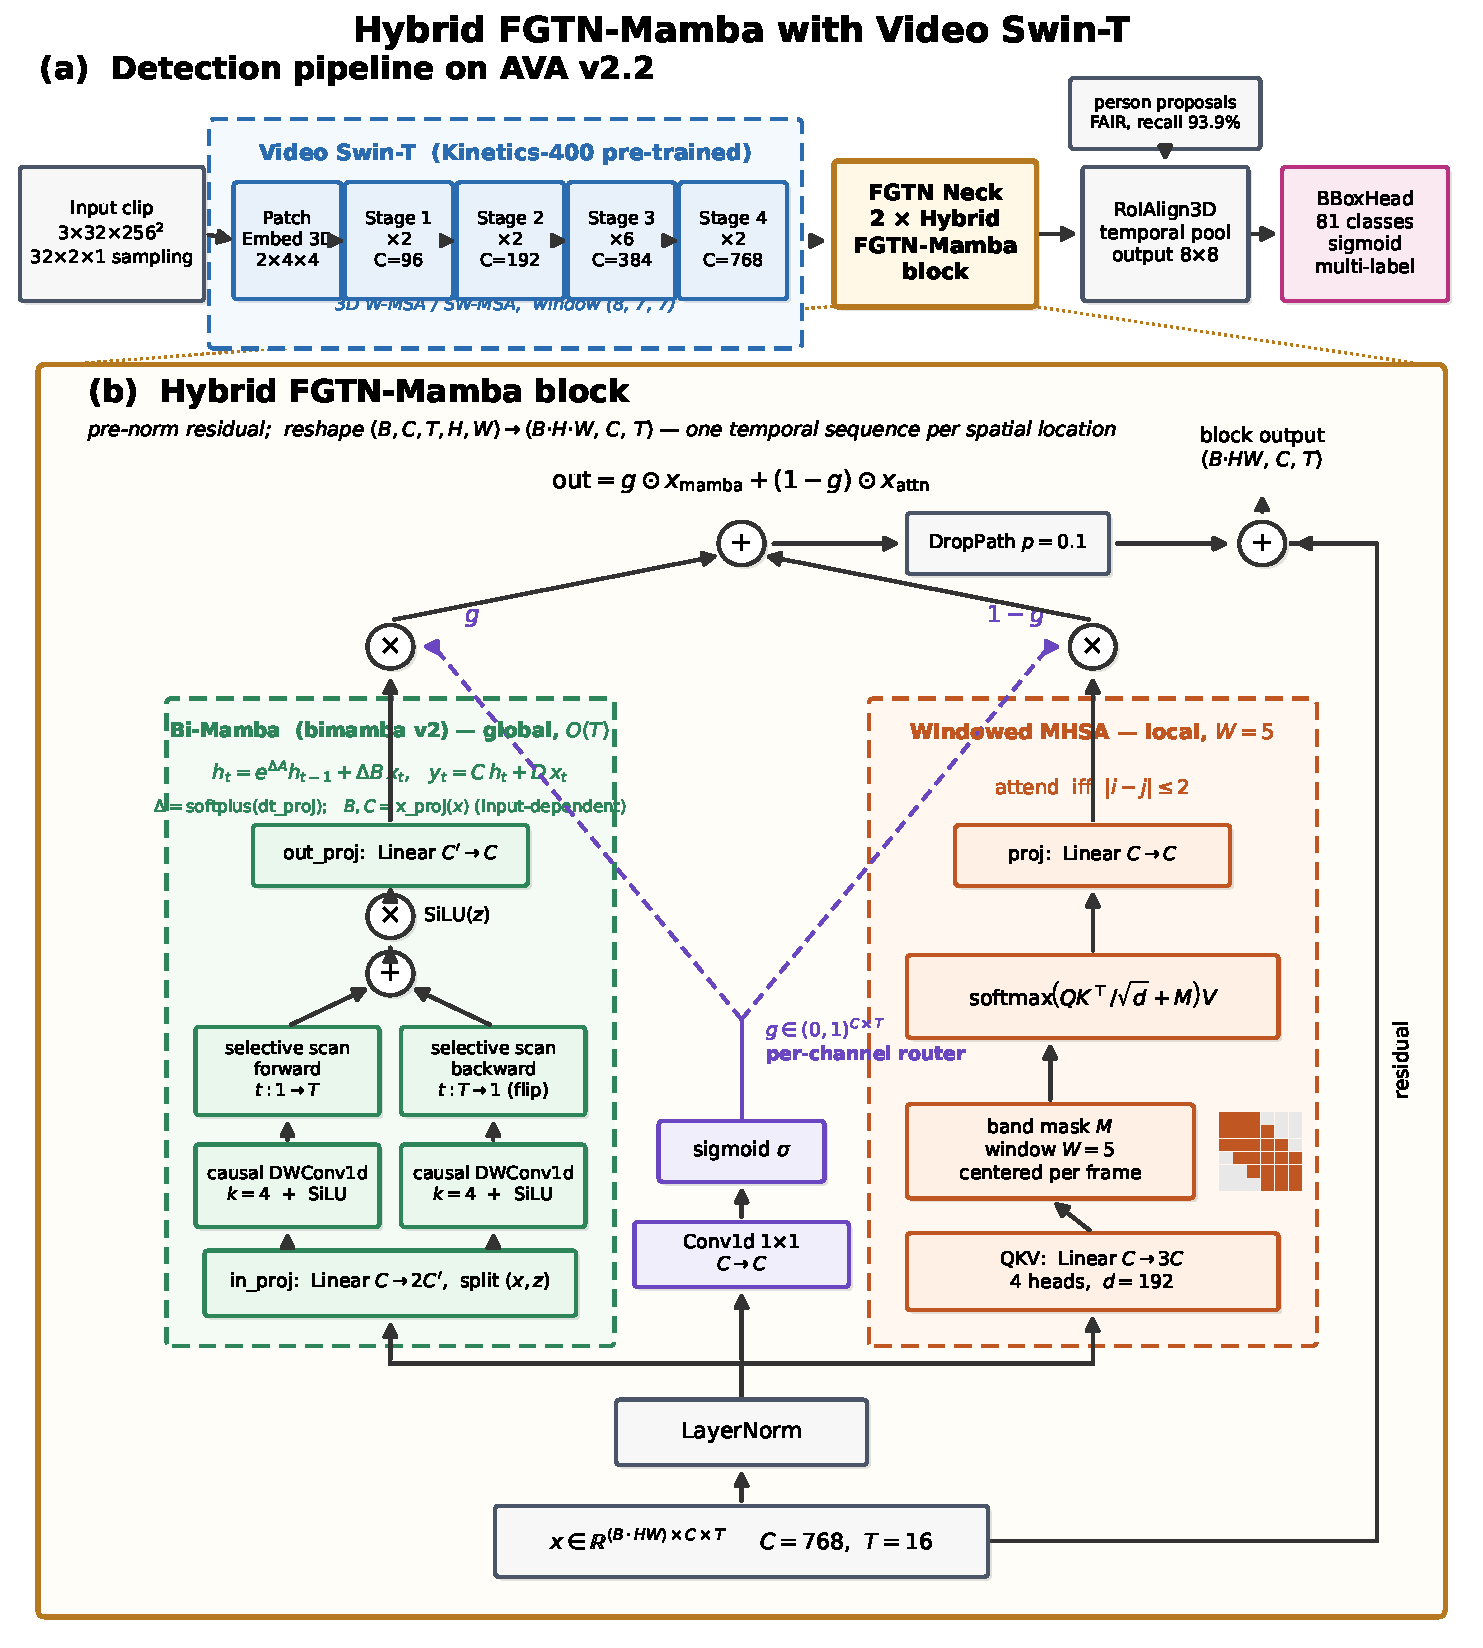
\includegraphics[width=\textwidth]{fgtn_architecture.pdf}
\caption[Biến thể một tỉ lệ và cấu trúc khối Hybrid FGTN-Mamba]{Biến thể một tỉ lệ và cấu trúc khối. (a) Pipeline một tỉ lệ: Video Swin-T $\rightarrow$ FGTN neck (hai khối Hybrid FGTN-Mamba) $\rightarrow$ RoIAlign3D $\rightarrow$ BBoxHead sigmoid đa nhãn; pipeline đầy đủ bổ sung nhánh tầng 3 và ACRN như \cref{fig:pipeline}. (b) Một khối Hybrid FGTN-Mamba: nhánh Bi-Mamba (selective scan hai chiều, $O(T)$), nhánh windowed MHSA (mặt nạ dải, $W = 5$) và cổng sigmoid theo kênh và bước thời gian, $\mathrm{out} = g \odot x_{\text{mamba}} + (1 - g) \odot x_{\text{attn}}$.}
\label{fig:architecture}
\end{figure}

\section{Vị trí đặt khối: hậu-backbone, tiền-RoI}
\label{sec:placement}

Khối được đặt sau backbone và trước 3D RoIAlign vì ba lý do. Nếu đặt bên trong Video Swin, phải sửa kiến trúc đã tiền huấn luyện và trọng số Kinetics-400 không còn nạp được nguyên vẹn. Nếu đặt sau RoIAlign, mô hình thời gian chỉ nhìn vùng người đã bị cắt, mất tín hiệu cảnh; hơn nữa \code{SingleRoIExtractor3D} gộp trung bình theo thời gian trước khi cắt nên trục $T$ không còn sau RoI. Khi đặt tiền-RoI, mỗi vị trí không gian được làm giàu bằng lịch sử dọc trục thời gian rồi RoIAlign mới lấy phần liên quan đến từng actor; giao diện ``tensor vào, tensor cùng kích thước ra'' cho phép thay backbone mà không đổi neck. Vị trí này cũng xác định phạm vi cải tiến: khối cải thiện biểu diễn theo thời gian, không sửa lỗi của person proposal và không tự giải quyết mất cân bằng dữ liệu.

\section{Đầu vào, định dạng lại và chuẩn hóa}
\label{sec:reshape}

Với bản đồ đặc trưng $F \in \R^{B \times C \times T \times H \times W}$, neck chỉ mô hình hóa dọc trục $T$, không trộn không gian thêm lần nữa. Tensor được hoán vị và định dạng lại thành
\begin{equation}
\mat{X} = \mathrm{reshape}\big(\mathrm{permute}(F)\big) \in \R^{(B \cdot H \cdot W) \times C \times T},
\label{eq:reshape}
\end{equation}
tức mỗi tọa độ không gian là một chuỗi độc lập gồm $T$ token $C$ chiều; sau các khối, tensor được đưa về dạng ban đầu. Mỗi khối dùng chuẩn hóa trước (pre-norm) trên chiều kênh tại từng bước thời gian:
\begin{equation}
\bar{\mat{X}} = \LN(\mat{X}), \qquad \epsilon = 10^{-6}.
\label{eq:prenorm}
\end{equation}
Ở tầng 4, $C = 768$, $T = 16$ (32 khung hình qua patch embedding thời gian bước 2), $H = W = 8$ và số chuỗi là $B \cdot 64$; ở tầng 3, $C = 384$, $H = W = 16$ và số chuỗi là $B \cdot 256$.

\section{Nhánh toàn cục: mô hình không gian trạng thái chọn lọc hai chiều}
\label{sec:ssm-branch}

Nhánh SSM nhắm vào L1 và L2 (\cref{tab:gaps}). Với hành vi bền vững như ngủ trên bàn hay gác chân, vài khung hình quanh khung hình khóa không đủ để phân biệt tư thế tạm thời với hành vi kéo dài; selective scan truyền một trạng thái qua toàn bộ chuỗi với số bước tuyến tính theo $T$. Nhánh dùng khối Mamba \cite{gu2023mamba} theo cài đặt \code{bimamba v2} của Video Mamba Suite \cite{chen2024videomambasuite}, với $N = 16$, hệ số mở rộng $E = 2$ ($C' = 2C$), hạng phép chiếu bước thời gian $\lceil C/16 \rceil$ và tích chập nhân quả theo kênh $k = 4$. Trên mỗi chuỗi $\bar{\mat{X}} \in \R^{T \times C}$:
\begin{align}
[\mat{U};\ \mat{Z}] &= \bar{\mat{X}}\mat{W}_{\text{in}}, \qquad \mat{U}, \mat{Z} \in \R^{T \times C'}, \label{eq:mamba-in}\\
\mat{U}' &= \mathrm{SiLU}\big(\mathrm{DWConv1d}_{k=4}(\mat{U})\big), \label{eq:mamba-conv}\\
\Delta_t &= \mathrm{softplus}\big(\mat{W}_\Delta \mat{W}_{\text{dt}} \mat{u}'_t + \mat{b}_\Delta\big), \quad
\mat{B}_t = \mat{W}_B \mat{u}'_t, \quad \mat{C}_t = \mat{W}_C \mat{u}'_t, \label{eq:mamba-sel}\\
\mat{h}_t &= \exp(\Delta_t \mat{A})\,\mat{h}_{t-1} + \Delta_t \mat{B}_t \mat{u}'_t, \qquad
y_t = \mat{C}_t^{\top}\mat{h}_t + D\,u'_t, \label{eq:mamba-scan}\\
\mat{S}^{\rightarrow} &= \mat{Y} \odot \mathrm{SiLU}(\mat{Z}). \label{eq:mamba-gate}
\end{align}
Ở đây $\mat{A} = -\exp(\mat{A}_{\log})$ là tham số học được, còn $\Delta_t$, $\mat{B}_t$, $\mat{C}_t$ sinh từ đầu vào tại mỗi bước, nên mức giữ/quên trạng thái thay đổi theo nội dung: đoạn gần như tĩnh duy trì trạng thái lâu hơn, thay đổi đột ngột làm tăng trọng số cho đầu vào mới. Tính chọn lọc này quan trọng hơn việc chỉ thay attention bằng một phép hồi quy, và phù hợp với dữ liệu có cả hành vi bền vững lẫn thao tác nhanh. Vì đoạn video lấy đối xứng quanh khung hình khóa, \code{bimamba v2} dùng thêm một bộ tham số quét riêng cho chiều ngược, dùng chung $\mat{W}_{\text{in}}$ và $\mat{W}_{\text{out}}$:
\begin{equation}
\mat{S}^{\leftarrow} = \mathrm{flip}\big(\Scan_b(\mathrm{flip}(\bar{\mat{X}}))\big), \qquad
\mat{S} = \tfrac{1}{2}\big(\mat{S}^{\rightarrow} + \mat{S}^{\leftarrow}\big)\mat{W}_{\text{out}} \in \R^{T \times C}.
\label{eq:bimamba}
\end{equation}
Quét ngược bổ sung các khung hình sau khung hình khóa, đổi lại hệ cảnh báo trực tuyến phải chịu độ trễ nhìn trước (look-ahead) tương ứng (\cref{sec:inference}).

\section{Nhánh cục bộ: self-attention trong cửa sổ thời gian}
\label{sec:local-branch}

SSM nén lịch sử vào trạng thái nên có thể làm mờ một chuyển tiếp rất ngắn, như pha đưa điện thoại lên hay bắt đầu một thao tác nguy hiểm. Nhánh cục bộ giữ đường so khớp trực tiếp giữa mỗi khung hình và các khung hình lân cận. Từ $\bar{\mat{X}}$, phép chiếu $\mat{W}_{\text{qkv}} \in \R^{C \times 3C}$ tạo $\mat{Q}, \mat{K}, \mat{V}$ chia thành $h = 4$ đầu; với $W = 5$, token $i$ chỉ chú ý tới token $j$ thỏa $|i - j| \leq 2$:
\begin{equation}
\mat{A}_{\text{loc}} = \softmax\!\left(\frac{\mat{Q}\mat{K}^{\top}}{\sqrt{d}} + \mat{M}\right)\mat{V}\,\mat{W}_{\text{proj}}, \qquad
M_{ij} = \begin{cases} 0, & |i - j| \leq 2,\\ -\infty, & \text{ngược lại.}\end{cases}
\label{eq:local-attn}
\end{equation}
Ở biên đoạn video, mặt nạ chỉ giữ các phần tử hợp lệ, không quấn vòng; bốn đầu cho phép các không gian con kênh học các kiểu chuyển động khác nhau. Vì $T = 16$ tại neck, ma trận $T \times T$ được tính rồi che với chi phí không đáng kể; khi $T$ lớn, cùng công thức có thể thực thi theo dạng dải với chi phí $O(TWC)$ \cite{beltagy2020longformer}. Nhánh cục bộ chưa dùng mã hóa vị trí tương đối; thứ tự thời gian được nhánh SSM cung cấp gián tiếp qua đường residual.

\section{Cổng sigmoid: định tuyến dài hạn--ngắn hạn theo nội dung}
\label{sec:gate}

Nếu cộng $\mat{S}$ và $\mat{A}_{\text{loc}}$ với trọng số cố định, mọi kênh và mọi đoạn video nhận cùng tỷ lệ dài hạn--ngắn hạn, mâu thuẫn với đặc thù các hành vi ở \cref{sec:behaviours}. Cổng sigmoid là bộ định tuyến mềm, tính từ đầu vào đã chuẩn hóa bằng tích chập $1 \times 1$ theo kênh:
\begin{equation}
\mat{G} = \sigma\big(\mat{W}_g \bar{\mat{X}} + \mat{b}_g\big) \in (0,1)^{C \times T}, \qquad
\mat{Z} = \mat{G} \odot \mat{S} + (\mat{1} - \mat{G}) \odot \mat{A}_{\text{loc}}.
\label{eq:gate}
\end{equation}
Cổng phụ thuộc nội dung, vị trí không gian, kênh và bước thời gian: cùng một kênh có thể ưu tiên trạng thái dài hạn ở pha tĩnh và chuyển sang nhánh cục bộ tại thời điểm chuyển tiếp; vì không chọn cứng, gradient vẫn truyền qua cả hai nhánh. Đầu ra khối là
\begin{equation}
\mat{Y} = \mat{X} + \mathrm{DropPath}_{p = 0{,}1}(\mat{Z}),
\label{eq:residual}
\end{equation}
với DropPath \cite{huang2016droppath} loại bỏ ngẫu nhiên toàn bộ nhánh dư của một chuỗi trong lúc huấn luyện; hai khối như vậy được xếp chồng.

Cùng một module cài đặt bốn chế độ qua tham số \code{branch\_mode}, phục vụ phần lớn ma trận ablation (\cref{tab:ablation}): \code{hybrid} theo \cref{eq:gate} (A6); \code{no\_gate} với $\mat{Z} = 0{,}5\,\mat{S} + 0{,}5\,\mat{A}_{\text{loc}}$ (A5); \code{mamba\_only} với $\mat{Z} = \mat{S}$ (A3); \code{attn\_only} với $\mat{Z} = \mat{A}_{\text{loc}}$ (A4). Temporal MHSA toàn cục (A1) là trường hợp riêng của \code{attn\_only} khi cửa sổ phủ toàn đoạn (\code{window\_size} $\geq 31$ với $T = 16$); baseline không neck (A0) tương ứng \code{model.neck = None}; SSM một chiều (A2) dùng \code{bimamba\_type = "none"} của \code{mamba-ssm}, hiện chưa có khóa cấu hình tương ứng.

\section{Ổn định huấn luyện và cài đặt dự phòng}
\label{sec:stability}

Pre-norm và residual cho phép khối học phần dư thay vì tái tạo toàn bộ bản đồ đặc trưng; ở khởi tạo, hai nhánh đóng góp nhỏ và pipeline xấp xỉ pipeline không có neck, nên trọng số tiền huấn luyện của backbone không bị phá vỡ. Gradient được cắt với chuẩn tối đa 40 theo công thức gốc của MMAction2 cho AVA; kernel selective scan CUDA của \code{mamba-ssm} được khóa phiên bản vì sai khác kernel có thể ảnh hưởng tốc độ và khả năng tái lập. Khi thư viện \code{mamba-ssm} không khả dụng (ví dụ kiểm thử trên CPU), mã nguồn cung cấp bản cài đặt thuần PyTorch \code{NaiveBiMamba} thực hiện đúng hồi quy \cref{eq:mamba-scan} bằng vòng lặp theo $T$ với hai bộ tham số xuôi/ngược; bản này tương đương về mặt số học nhưng chậm hơn khoảng hai bậc, chỉ dùng để kiểm tra kích thước tensor.

\section{Độ phức tạp và so sánh với các temporal neck khác}
\label{sec:complexity}

Xét chuỗi độ dài $T$, $C$ kênh, cửa sổ $W$, trạng thái $N$ và hệ số mở rộng $E$. Trong một khối, nhánh SSM tốn $O(T \cdot C \cdot EC)$ cho các phép chiếu, $O(T \cdot EC \cdot k)$ cho tích chập và $O(T \cdot EC \cdot N)$ cho selective scan mỗi chiều; nhánh cục bộ tốn $O(T \cdot C^2)$ cho phép chiếu và $O(T \cdot W \cdot C)$ cho so khớp trong cửa sổ; cổng tốn $O(T \cdot C^2)$. Mọi số hạng đều tuyến tính theo $T$: tổng chi phí là $O\big(T(C^2 + CN + WC)\big)$ và phần phụ thuộc cấu trúc thời gian là $O(TC + TWC)$, thay vì $O(T^2 C)$ của attention toàn cục (\cref{tab:necks}). Chi phí toàn neck nhân với số chuỗi $B \cdot H \cdot W$, nên tầng 3 ($16 \times 16$) tốn gấp bốn lần tầng 4.

\begin{table}[htbp]
\centering
\caption{So sánh các temporal neck tại cùng vị trí hậu-backbone}
\label{tab:necks}
\small
\begin{tabularx}{\textwidth}{lXlX}
\toprule
\textbf{Cơ chế} & \textbf{Nội dung} & \textbf{Chi phí theo $T$} & \textbf{Đặc tính}\\
\midrule
Temporal MHSA toàn cục & So khớp mọi cặp khung hình & $O(T^2 C)$ & Toàn cục nhưng bộ nhớ tăng nhanh\\
Tích chập thời gian / TPN \cite{yang2020tpn} & Nhân, hệ số giãn cố định & $O(T k C^2)$ & Thiên lệch cục bộ; trường tiếp nhận theo độ sâu\\
SSM thuần \cite{li2024videomamba} & Selective scan & $O(TC)$ & Dài hạn tốt; có thể thiếu chuyển tiếp cục bộ\\
Hybrid FGTN-Mamba & Bi-SSM + W-MHSA + cổng & $O(TC + TWC)$ & Dài--ngắn tách nhánh, định tuyến theo nội dung\\
\bottomrule
\end{tabularx}
\end{table}

\Cref{tab:params} tổng hợp số tham số theo cấu trúc của neck. Với $C = 768$, một khối có 6.957.312 tham số (nhánh Mamba 4.002.816, nhánh attention 2.362.368, cổng 590.592); neck hai khối có 13.914.624 tham số, khoảng một nửa backbone Video Swin-T (27.850.470). Pipeline đầy đủ thêm khoảng 3,57 triệu tham số cho ngăn xếp tầng 3 và khoảng 14,6 triệu cho ACRN. Ngoài chi phí tuyến tính, khối đưa vào ba thiên lệch quy nạp phù hợp bài toán: trạng thái có thứ tự cho diễn biến dài, so khớp cục bộ cho chuyển tiếp ngắn và bộ định tuyến theo nội dung.

\begin{table}[htbp]
\centering
\caption{Số tham số theo cấu trúc của neck một tỉ lệ ($C = 768$, hai khối)}
\label{tab:params}
\begin{tabularx}{\textwidth}{Xrr}
\toprule
\textbf{Thành phần (mỗi khối)} & \textbf{Kích thước chính} & \textbf{Tham số}\\
\midrule
LayerNorm & $2 \times 768$ & 1.536\\
Mamba: \code{in\_proj} & $3072 \times 768$ & 2.359.296\\
Mamba: hai bộ quét (conv1d, \code{x\_proj}, \code{dt\_proj}, $\mat{A}_{\log}$, $D$) & $2 \times 231.936$ & 463.872\\
Mamba: \code{out\_proj} & $768 \times 1536$ & 1.179.648\\
W-MHSA: \code{qkv} + \code{proj} & $2304 \times 768$, $768 \times 768$ & 2.362.368\\
Cổng: Conv1d $1 \times 1$ & $768 \times 768$ & 590.592\\
\midrule
Một khối & & 6.957.312\\
Neck (hai khối) & & 13.914.624\\
\bottomrule
\end{tabularx}
\end{table}

\section{Thành phần tích hợp 1: đặc trưng đa tỉ lệ}
\label{sec:multiscale}

Thành phần này xử lý L3. Video Swin-T tạo bốn tầng đặc trưng với $96, 192, 384, 768$ kênh và bước giảm mẫu $4, 8, 16, 32$. Chỉ dùng tầng 4 thì điện thoại hay bàn chân chiếm chưa đến một ô trên lưới $8 \times 8$. Pipeline đầy đủ đặt \code{out\_indices = (2, 3)} để lấy thêm tầng 3 và tạo \emph{một ngăn xếp Hybrid FGTN-Mamba riêng cho mỗi tầng} (\code{in\_channels = (384, 768)}), không chia sẻ tham số. Sau neck, \code{SingleRoIExtractor3D} nội suy bản đồ tầng 4 về độ phân giải tầng 3, gộp trung bình theo thời gian, nối theo kênh và cắt RoI với tỷ lệ $1/16$:
\begin{equation}
r_k = \RoIAlign\Big(\Concat\big[\Pool_T(\tilde{F}^{(3)}),\ \Pool_T(\uparrow_2 \tilde{F}^{(4)})\big],\ b_k\Big) \in \R^{1152 \times 1 \times 8 \times 8}.
\label{eq:multiscale}
\end{equation}
Gộp theo thời gian được thực hiện có chủ đích \emph{sau} khi mỗi tầng đã nhận ngữ cảnh dài--ngắn từ neck. Tầng 3 có số chuỗi thời gian gấp bốn tầng 4, nên kích thước lô của cấu hình đa tỉ lệ cần được lựa chọn theo bộ nhớ khả dụng; cặp A6 $\rightarrow$ A7 tách đóng góp của thành phần này.

\section{Thành phần tích hợp 2: mạng quan hệ actor--cảnh (ACRN)}
\label{sec:acrn}

ACRN \cite{sun2018acrn} xử lý L4: trong phân xưởng, cùng một tư thế mang ý nghĩa khác nhau tùy theo bàn, ghế, thiết bị xung quanh người. Luận văn dùng \code{ACRNHead} của MMAction2 làm \code{shared\_head} trong \code{AVARoIHead}. Với đặc trưng RoI $r_k$ và bản đồ cảnh $G$ (đã gộp theo thời gian, $1152 \times 1 \times h \times w$):
\begin{multline}
c_k = \mathrm{Conv}_{1\times3\times3}\Big(\mathrm{Conv}_{1\times1\times1}\big(\Concat[\Tile_{h \times w}(\max\!\Pool(r_k)),\ G_{\text{batch}(k)}]\big)\Big)\\
\in \R^{1152 \times 1 \times h \times w},
\label{eq:acrn}
\end{multline}
trong đó mỗi tích chập kèm BatchNorm và ReLU. Vectơ actor được lát (tile) lên toàn bộ lưới cảnh, nên quan hệ được điều kiện theo từng actor: hai người trong cùng khung hình nhận ngữ cảnh khác nhau. So với gộp trung bình toàn cục, ACRN giữ bố cục không gian của cảnh; so với STAR \cite{gritsenko2024star}, nó vẫn phụ thuộc proposal nhưng tích hợp trực tiếp vào pipeline hai giai đoạn.

\section{Thành phần tích hợp 3: hàm mất mát hai cấp và ngưỡng theo lớp}
\label{sec:loss}

Head \code{BBoxHeadAVA} của MMAction2 chỉ giữ các RoI có ít nhất một nhãn dương ($\mathcal{P}$) và tính BCE trên $K$ logit sigmoid:
\begin{equation}
\mathcal{L}_{\text{BCE}} = \frac{1}{|\mathcal{P}| \cdot K} \sum_{k \in \mathcal{P}} \sum_{c=1}^{K}
  \BCE\big(s_{k,c}, y_{k,c}\big).
\label{eq:bce}
\end{equation}
Thành phần này xử lý L5: head \code{BBoxHeadAVAWeighted} giữ nguyên phần chọn RoI và chỉ thay biểu thức mất mát bằng focal loss có trọng số lớp,
\begin{equation}
\begin{gathered}
\mathcal{L} = \frac{1}{|\mathcal{P}| \cdot K} \sum_{k \in \mathcal{P}} \sum_{c=1}^{K}
  w_c\, \alpha\, (1 - p_{t,k,c})^{\gamma}\, \BCE(s_{k,c}, y_{k,c}),\\
p_{t,k,c} = \exp\big(-\BCE(s_{k,c}, y_{k,c})\big),
\end{gathered}
\label{eq:focal}
\end{equation}
với $\gamma = 2$, $\alpha = 1$; khi $\gamma = 0$ và $w_c = 1$, \cref{eq:focal} trùng với \cref{eq:bce}. Trọng số lớp tính theo số mẫu hiệu dụng \cite{cui2019classbalanced}:
\begin{equation}
w_c = \frac{\tilde{w}_c}{\frac{1}{K}\sum_{c'} \tilde{w}_{c'}}, \qquad
\tilde{w}_c = \frac{1 - \beta}{1 - \beta^{\max(n_c, 1)}}, \qquad \beta = 0{,}999,
\label{eq:classweight}
\end{equation}
được chuẩn hóa để trung bình bằng 1 và cắt trên tại 10. Sau huấn luyện, ngưỡng $\tau_c$ của từng lớp được chọn trên tập kiểm định theo tiêu chí nghiệp vụ (ví dụ cực đại F1 hoặc đạt recall tối thiểu); mAP không phụ thuộc ngưỡng nên không bị ảnh hưởng bởi lựa chọn này.

\section{Luồng suy luận và logic cảnh báo}
\label{sec:inference}

\begin{enumerate}
  \item Lấy đoạn 32 khung hình (bước 2) đối xứng quanh khung hình khóa, đổi kích thước cạnh ngắn về 256; đọc person proposal (hoặc chạy bộ phát hiện người).
  \item Trích đặc trưng tầng 3 và tầng 4, chạy Hybrid FGTN-Mamba riêng trên từng tầng, 3D RoIAlign đa tỉ lệ, ACRN và head sigmoid cho $p_{k,c}$.
  \item So $p_{k,c}$ với $\tau_c$; chỉ phát sự kiện khi cùng actor vượt ngưỡng $m$ trong $n$ khung hình khóa liên tiếp, giảm cảnh báo chớp tắt.
  \item Ghép sự kiện theo định danh track, lưu thời điểm, hộp, lớp, điểm và ảnh minh chứng; áp dụng thời gian chờ (cooldown) để tránh lặp cảnh báo.
\end{enumerate}
Các tham số $m/n$, cooldown và $\tau_c$ thuộc lớp nghiệp vụ, không được tối ưu trên tập kiểm tra. Độ trễ đầu--cuối gồm giải mã, bộ phát hiện người, bộ đệm nhìn trước của quét hai chiều (tối thiểu nửa đoạn video), mô hình và gửi cảnh báo; thời gian suy luận của riêng mô hình không đại diện cho toàn hệ thống. \Cref{tab:shapes} tóm tắt kích thước tensor qua pipeline.

\begin{table}[H]
\centering
\caption{Chuỗi kích thước đặc trưng với ảnh cắt $256 \times 256$, 32 khung hình đầu vào}
\label{tab:shapes}
\small
\begin{tabularx}{\textwidth}{llX}
\toprule
\textbf{Khối} & \textbf{Kích thước} & \textbf{Ghi chú}\\
\midrule
Đầu vào & $B \times 3 \times 32 \times 256 \times 256$ & Đoạn RGB\\
Patch embedding $(2, 4, 4)$ & $B \times 96 \times 16 \times 64 \times 64$ & $T = 16$ từ đây\\
Swin tầng 3 & $B \times 384 \times 16 \times 16 \times 16$ & Chỉ trong pipeline đa tỉ lệ\\
Swin tầng 4 & $B \times 768 \times 16 \times 8 \times 8$ & Cả hai biến thể\\
Neck (mỗi tầng) & giữ nguyên kích thước & Mô hình hóa thời gian theo từng vị trí\\
RoI tầng 4 (một tỉ lệ) & $N \times 768 \times 1 \times 8 \times 8$ & Gộp trung bình theo $T$ trước khi cắt\\
RoI đa tỉ lệ & $N \times 1152 \times 1 \times 8 \times 8$ & Nối $384 + 768$ tại tỷ lệ $1/16$\\
ACRN & $N \times 1152 \times 1 \times 16 \times 16$ & Lưới cảnh tầng 3\\
Head & $N \times (K + 1)$ & $K$ lớp $+$ nền ($K = 4$ hoặc 80)\\
\bottomrule
\end{tabularx}
\end{table}

\section{Rủi ro kỹ thuật và cách giám sát}
\label{sec:risks}

\begin{itemize}
  \item \emph{Cổng bão hòa}: $g$ dồn về một nhánh; theo dõi phân bố $g$ và chuẩn gradient từng nhánh theo epoch.
  \item \emph{Tầng lấn át}: tầng 4 lấn tầng 3 trong cấu hình đa tỉ lệ; đo chuẩn đặc trưng và ablation từng tầng.
  \item \emph{Điểm nóng bộ nhớ}: tầng 3 tạo $B \cdot 256$ chuỗi; theo dõi bộ nhớ đỉnh theo lô, $T$ và độ phân giải.
  \item \emph{Độ trễ hai chiều}: quét ngược cần khung hình tương lai; báo cả thông lượng và độ trễ đầu--cuối.
  \item \emph{Sai lệch tỷ lệ RoI}: \code{featmap\_stride} của bộ trích RoI phải khớp bước giảm mẫu của bản đồ đặc trưng (32 với tầng 4, 16 với cấu hình đa tỉ lệ).
  \item \emph{Bão hòa độ đo}: với dữ liệu nhỏ, mAP cao có thể che khuất lỗi; cần kiểm tra theo camera (cách chia S2, \cref{sec:splits}), mẫu âm khó và sai số hiệu chỉnh.
\end{itemize}

\section*{Tiểu kết chương}
\addcontentsline{toc}{section}{Tiểu kết chương}

Chương này đã mô tả Hybrid FGTN-Mamba gồm nhánh Bi-SSM cho phụ thuộc dài hạn, nhánh W-MHSA cho chuyển tiếp ngắn hạn và cổng sigmoid định tuyến theo kênh và bước thời gian, với chi phí tuyến tính theo độ dài chuỗi; khối được đặt tại vị trí hậu-backbone, tiền-RoI và áp dụng độc lập trên hai tầng đặc trưng. Pipeline đầy đủ bổ sung multi-scale RoI, ACRN, hàm mất mát hai cấp và logic cảnh báo theo track. Các chế độ nhánh của cùng một module cho phép hiện thực phần lớn ma trận ablation trình bày trong \cref{ch:experiments}.
